\documentclass{standalone}
\usepackage{tikz}
\usetikzlibrary{patterns, positioning}

\begin{document}
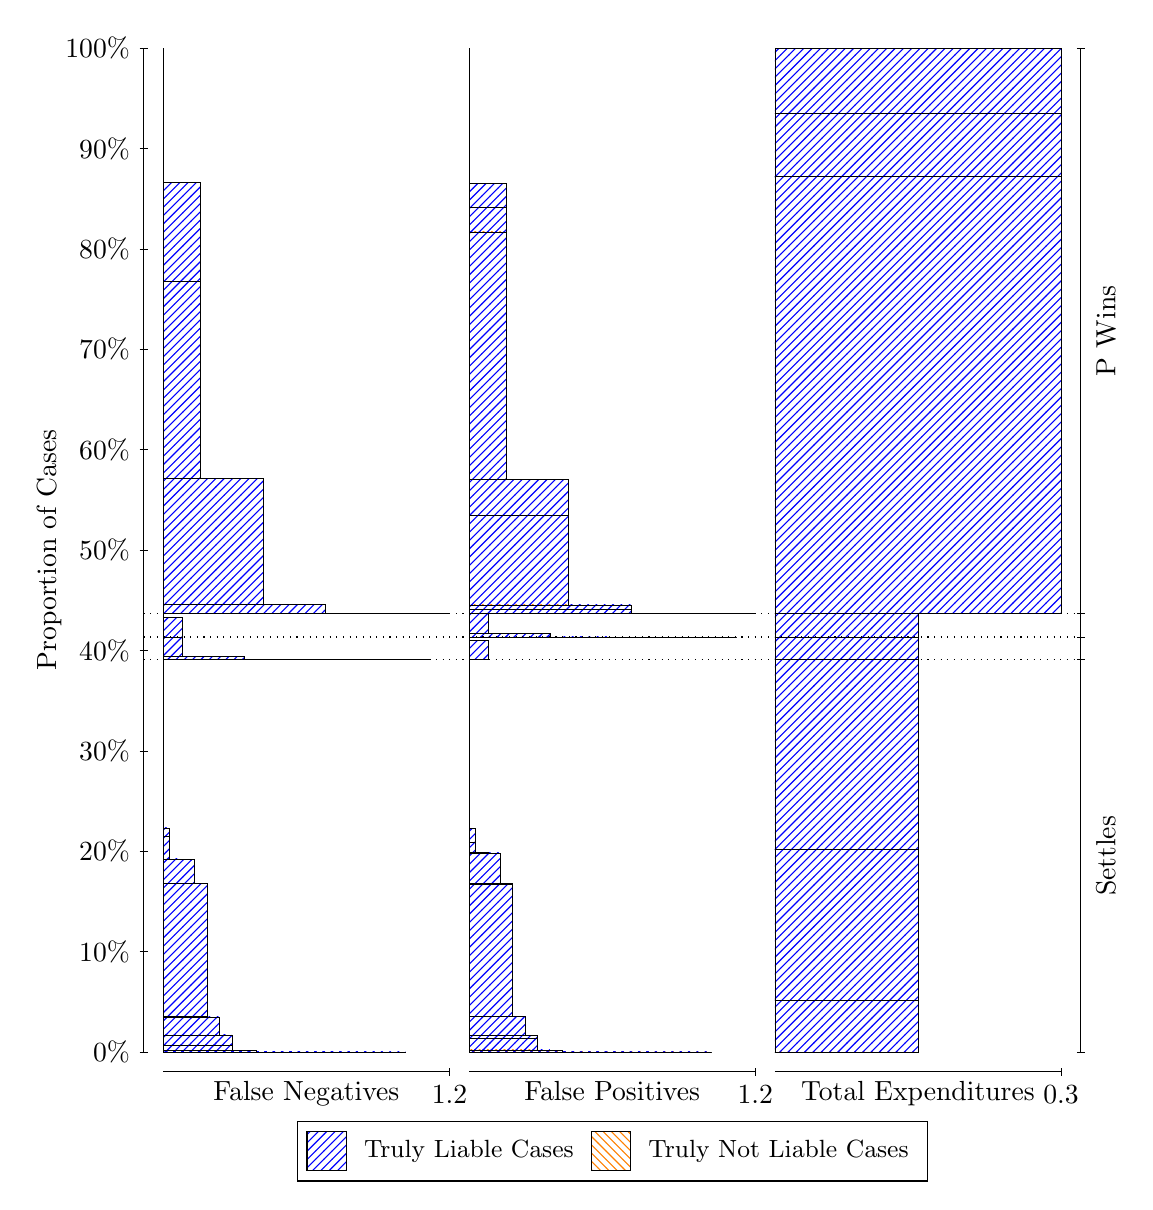
\begin{tikzpicture}
\draw[black, very thin] (1.5,1.75) -- (1.5,14.5);
\node[rotate=90, anchor=center] at (0.3, 8.125) {Proportion of Cases};
\draw[black, very thin] (1.45,1.75) -- (1.55,1.75);
\node[anchor=east] at (1.45, 1.75) {0\%};
\draw[black, very thin] (1.45,3.025) -- (1.55,3.025);
\node[anchor=east] at (1.45, 3.025) {10\%};
\draw[black, very thin] (1.45,4.3) -- (1.55,4.3);
\node[anchor=east] at (1.45, 4.3) {20\%};
\draw[black, very thin] (1.45,5.575) -- (1.55,5.575);
\node[anchor=east] at (1.45, 5.575) {30\%};
\draw[black, very thin] (1.45,6.85) -- (1.55,6.85);
\node[anchor=east] at (1.45, 6.85) {40\%};
\draw[black, very thin] (1.45,8.125) -- (1.55,8.125);
\node[anchor=east] at (1.45, 8.125) {50\%};
\draw[black, very thin] (1.45,9.4) -- (1.55,9.4);
\node[anchor=east] at (1.45, 9.4) {60\%};
\draw[black, very thin] (1.45,10.675) -- (1.55,10.675);
\node[anchor=east] at (1.45, 10.675) {70\%};
\draw[black, very thin] (1.45,11.95) -- (1.55,11.95);
\node[anchor=east] at (1.45, 11.95) {80\%};
\draw[black, very thin] (1.45,13.225) -- (1.55,13.225);
\node[anchor=east] at (1.45, 13.225) {90\%};
\draw[black, very thin] (1.45,14.5) -- (1.55,14.5);
\node[anchor=east] at (1.45, 14.5) {100\%};

\draw[black, very thin] (13.4,1.75) -- (13.4,14.5);
\draw[black, very thin] (13.35,1.75) -- (13.45,1.75);
\node[anchor=west] at (13.35, 1.75) {};
\draw[black, very thin] (13.35,6.7316) -- (13.45,6.7316);
\node[anchor=west] at (13.35, 6.7316) {};
\draw[black, very thin] (13.35,7.0198) -- (13.45,7.0198);
\node[anchor=west] at (13.35, 7.0198) {};
\draw[black, very thin] (13.35,7.3156) -- (13.45,7.3156);
\node[anchor=west] at (13.35, 7.3156) {};
\draw[black, very thin] (13.35,14.5) -- (13.45,14.5);
\node[anchor=west] at (13.35, 14.5) {};

\draw[black, very thin, pattern color=blue, pattern=north east lines] (1.75,1.75) rectangle (4.8304,1.75);
\draw[black, very thin, pattern color=blue, pattern=north east lines] (1.75,1.75) rectangle (4.5145,1.75);
\draw[black, very thin, pattern color=blue, pattern=north east lines] (1.75,1.75) rectangle (4.1986,1.75);
\draw[black, very thin, pattern color=blue, pattern=north east lines] (1.75,1.75) rectangle (4.0406,1.75);
\draw[black, very thin, pattern color=blue, pattern=north east lines] (1.75,1.75) rectangle (3.8826,1.75);
\draw[black, very thin, pattern color=blue, pattern=north east lines] (1.75,1.75) rectangle (3.7246,1.75);
\draw[black, very thin, pattern color=blue, pattern=north east lines] (1.75,1.75) rectangle (3.5667,1.75);
\draw[black, very thin, pattern color=blue, pattern=north east lines] (1.75,1.75) rectangle (3.4087,1.7504);
\draw[black, very thin, pattern color=blue, pattern=north east lines] (1.75,1.7504) rectangle (3.2507,1.752);
\draw[black, very thin, pattern color=blue, pattern=north east lines] (1.75,1.752) rectangle (3.0928,1.752);
\draw[black, very thin, pattern color=blue, pattern=north east lines] (1.75,1.752) rectangle (3.0928,1.7522);
\draw[black, very thin, pattern color=blue, pattern=north east lines] (1.75,1.7522) rectangle (2.9348,1.7687);
\draw[black, very thin, pattern color=blue, pattern=north east lines] (1.75,1.7687) rectangle (2.7768,1.7691);
\draw[black, very thin, pattern color=blue, pattern=north east lines] (1.75,1.7691) rectangle (2.6188,1.8406);
\draw[black, very thin, pattern color=blue, pattern=north east lines] (1.75,1.8406) rectangle (2.6188,1.9663);
\draw[black, very thin, pattern color=blue, pattern=north east lines] (1.75,1.9663) rectangle (2.4609,2.1954);
\draw[black, very thin, pattern color=blue, pattern=north east lines] (1.75,2.1954) rectangle (2.3029,2.1955);
\draw[black, very thin, pattern color=blue, pattern=north east lines] (1.75,2.1955) rectangle (2.3029,2.2004);
\draw[black, very thin, pattern color=blue, pattern=north east lines] (1.75,2.2004) rectangle (2.3029,3.8891);
\draw[black, very thin, pattern color=blue, pattern=north east lines] (1.75,3.8891) rectangle (2.1449,4.1925);
\draw[black, very thin, pattern color=blue, pattern=north east lines] (1.75,4.1925) rectangle (1.987,4.2036);
\draw[black, very thin, pattern color=blue, pattern=north east lines] (1.75,4.2036) rectangle (1.829,4.4862);
\draw[black, very thin, pattern color=blue, pattern=north east lines] (1.75,4.4862) rectangle (1.829,4.5952);
\draw[black, very thin, pattern color=orange, pattern=north west lines] (1.75,4.5952) rectangle (1.75,4.5952);
\draw[black, very thin, pattern color=blue, pattern=north east lines] (1.75,4.5952) rectangle (1.75,6.7316);
\draw[black, very thin, pattern color=blue, pattern=north east lines] (1.75,6.7316) rectangle (5.1464,6.7316);
\draw[black, very thin, pattern color=blue, pattern=north east lines] (1.75,6.7316) rectangle (4.3565,6.7316);
\draw[black, very thin, pattern color=blue, pattern=north east lines] (1.75,6.7316) rectangle (3.5667,6.7319);
\draw[black, very thin, pattern color=blue, pattern=north east lines] (1.75,6.7319) rectangle (2.7768,6.776);
\draw[black, very thin, pattern color=blue, pattern=north east lines] (1.75,6.776) rectangle (1.987,7.0198);
\draw[black, very thin, pattern color=orange, pattern=north west lines] (1.75,7.0198) rectangle (1.75,7.0198);
\draw[black, very thin, pattern color=blue, pattern=north east lines] (1.75,7.0198) rectangle (1.987,7.2699);
\draw[black, very thin, pattern color=orange, pattern=north west lines] (1.75,7.2699) rectangle (1.75,7.2699);
\draw[black, very thin, pattern color=blue, pattern=north east lines] (1.75,7.2699) rectangle (1.75,7.3156);
\draw[black, very thin, pattern color=blue, pattern=north east lines] (1.75,7.3156) rectangle (5.3833,7.3156);
\draw[black, very thin, pattern color=blue, pattern=north east lines] (1.75,7.3156) rectangle (4.5935,7.3168);
\draw[black, very thin, pattern color=blue, pattern=north east lines] (1.75,7.3168) rectangle (3.8036,7.4297);
\draw[black, very thin, pattern color=blue, pattern=north east lines] (1.75,7.4297) rectangle (3.0138,9.0312);
\draw[black, very thin, pattern color=blue, pattern=north east lines] (1.75,9.0312) rectangle (2.2239,11.535);
\draw[black, very thin, pattern color=blue, pattern=north east lines] (1.75,11.535) rectangle (2.2239,12.789);
\draw[black, very thin, pattern color=orange, pattern=north west lines] (1.75,12.789) rectangle (1.75,12.789);
\draw[black, very thin, pattern color=blue, pattern=north east lines] (1.75,12.789) rectangle (1.75,14.5);
\draw[black, very thin, pattern color=orange, pattern=north west lines] (5.6333,1.75) rectangle (8.7138,1.75);
\draw[black, very thin, pattern color=blue, pattern=north east lines] (5.6333,1.75) rectangle (8.7138,1.75);
\draw[black, very thin, pattern color=orange, pattern=north west lines] (5.6333,1.75) rectangle (8.3978,1.75);
\draw[black, very thin, pattern color=blue, pattern=north east lines] (5.6333,1.75) rectangle (8.3978,1.75);
\draw[black, very thin, pattern color=orange, pattern=north west lines] (5.6333,1.75) rectangle (8.0819,1.75);
\draw[black, very thin, pattern color=blue, pattern=north east lines] (5.6333,1.75) rectangle (8.0819,1.75);
\draw[black, very thin, pattern color=blue, pattern=north east lines] (5.6333,1.75) rectangle (7.9239,1.75);
\draw[black, very thin, pattern color=orange, pattern=north west lines] (5.6333,1.75) rectangle (7.7659,1.75);
\draw[black, very thin, pattern color=blue, pattern=north east lines] (5.6333,1.75) rectangle (7.7659,1.75);
\draw[black, very thin, pattern color=blue, pattern=north east lines] (5.6333,1.75) rectangle (7.608,1.75);
\draw[black, very thin, pattern color=orange, pattern=north west lines] (5.6333,1.75) rectangle (7.45,1.75);
\draw[black, very thin, pattern color=blue, pattern=north east lines] (5.6333,1.75) rectangle (7.45,1.75);
\draw[black, very thin, pattern color=blue, pattern=north east lines] (5.6333,1.75) rectangle (7.292,1.7502);
\draw[black, very thin, pattern color=orange, pattern=north west lines] (5.6333,1.7502) rectangle (7.1341,1.7502);
\draw[black, very thin, pattern color=blue, pattern=north east lines] (5.6333,1.7502) rectangle (7.1341,1.7502);
\draw[black, very thin, pattern color=orange, pattern=north west lines] (5.6333,1.7502) rectangle (7.1341,1.7502);
\draw[black, very thin, pattern color=blue, pattern=north east lines] (5.6333,1.7502) rectangle (7.1341,1.7519);
\draw[black, very thin, pattern color=blue, pattern=north east lines] (5.6333,1.7519) rectangle (6.9761,1.752);
\draw[black, very thin, pattern color=orange, pattern=north west lines] (5.6333,1.752) rectangle (6.8181,1.752);
\draw[black, very thin, pattern color=blue, pattern=north east lines] (5.6333,1.752) rectangle (6.8181,1.7749);
\draw[black, very thin, pattern color=blue, pattern=north east lines] (5.6333,1.7749) rectangle (6.6601,1.7753);
\draw[black, very thin, pattern color=orange, pattern=north west lines] (5.6333,1.7753) rectangle (6.5022,1.7753);
\draw[black, very thin, pattern color=blue, pattern=north east lines] (5.6333,1.7753) rectangle (6.5022,1.9189);
\draw[black, very thin, pattern color=blue, pattern=north east lines] (5.6333,1.9189) rectangle (6.5022,1.9625);
\draw[black, very thin, pattern color=blue, pattern=north east lines] (5.6333,1.9625) rectangle (6.3442,1.9627);
\draw[black, very thin, pattern color=blue, pattern=north east lines] (5.6333,1.9627) rectangle (6.3442,2.2058);
\draw[black, very thin, pattern color=orange, pattern=north west lines] (5.6333,2.2058) rectangle (6.1862,2.2058);
\draw[black, very thin, pattern color=blue, pattern=north east lines] (5.6333,2.2058) rectangle (6.1862,3.8828);
\draw[black, very thin, pattern color=blue, pattern=north east lines] (5.6333,3.8828) rectangle (6.1862,3.8864);
\draw[black, very thin, pattern color=blue, pattern=north east lines] (5.6333,3.8864) rectangle (6.0283,4.278);
\draw[black, very thin, pattern color=blue, pattern=north east lines] (5.6333,4.278) rectangle (5.8703,4.2891);
\draw[black, very thin, pattern color=blue, pattern=north east lines] (5.6333,4.2891) rectangle (5.7123,4.4136);
\draw[black, very thin, pattern color=blue, pattern=north east lines] (5.6333,4.4136) rectangle (5.7123,4.5925);
\draw[black, very thin, pattern color=blue, pattern=north east lines] (5.6333,4.5925) rectangle (5.6333,6.7316);
\draw[black, very thin, pattern color=orange, pattern=north west lines] (5.6333,6.7316) rectangle (5.8703,6.7316);
\draw[black, very thin, pattern color=blue, pattern=north east lines] (5.6333,6.7316) rectangle (5.8703,6.9754);
\draw[black, very thin, pattern color=blue, pattern=north east lines] (5.6333,6.9754) rectangle (5.6333,7.0198);
\draw[black, very thin, pattern color=orange, pattern=north west lines] (5.6333,7.0198) rectangle (9.0297,7.0198);
\draw[black, very thin, pattern color=blue, pattern=north east lines] (5.6333,7.0198) rectangle (9.0297,7.0198);
\draw[black, very thin, pattern color=blue, pattern=north east lines] (5.6333,7.0198) rectangle (8.2399,7.0198);
\draw[black, very thin, pattern color=blue, pattern=north east lines] (5.6333,7.0198) rectangle (7.45,7.0202);
\draw[black, very thin, pattern color=blue, pattern=north east lines] (5.6333,7.0202) rectangle (6.6601,7.0656);
\draw[black, very thin, pattern color=blue, pattern=north east lines] (5.6333,7.0656) rectangle (5.8703,7.3156);
\draw[black, very thin, pattern color=orange, pattern=north west lines] (5.6333,7.3156) rectangle (9.2667,7.3156);
\draw[black, very thin, pattern color=blue, pattern=north east lines] (5.6333,7.3156) rectangle (9.2667,7.3156);
\draw[black, very thin, pattern color=orange, pattern=north west lines] (5.6333,7.3156) rectangle (8.4768,7.3156);
\draw[black, very thin, pattern color=blue, pattern=north east lines] (5.6333,7.3156) rectangle (8.4768,7.3159);
\draw[black, very thin, pattern color=blue, pattern=north east lines] (5.6333,7.3159) rectangle (8.4768,7.3167);
\draw[black, very thin, pattern color=orange, pattern=north west lines] (5.6333,7.3167) rectangle (7.687,7.3167);
\draw[black, very thin, pattern color=blue, pattern=north east lines] (5.6333,7.3167) rectangle (7.687,7.3733);
\draw[black, very thin, pattern color=blue, pattern=north east lines] (5.6333,7.3733) rectangle (7.687,7.4271);
\draw[black, very thin, pattern color=orange, pattern=north west lines] (5.6333,7.4271) rectangle (6.8971,7.4271);
\draw[black, very thin, pattern color=blue, pattern=north east lines] (5.6333,7.4271) rectangle (6.8971,8.563);
\draw[black, very thin, pattern color=blue, pattern=north east lines] (5.6333,8.563) rectangle (6.8971,9.0266);
\draw[black, very thin, pattern color=blue, pattern=north east lines] (5.6333,9.0266) rectangle (6.1072,12.166);
\draw[black, very thin, pattern color=orange, pattern=north west lines] (5.6333,12.166) rectangle (6.1072,12.166);
\draw[black, very thin, pattern color=blue, pattern=north east lines] (5.6333,12.166) rectangle (6.1072,12.473);
\draw[black, very thin, pattern color=blue, pattern=north east lines] (5.6333,12.473) rectangle (6.1072,12.784);
\draw[black, very thin, pattern color=blue, pattern=north east lines] (5.6333,12.784) rectangle (5.6333,14.5);
\draw[black, very thin, pattern color=orange, pattern=north west lines] (9.5167,1.75) rectangle (11.333,1.75);
\draw[black, very thin, pattern color=blue, pattern=north east lines] (9.5167,1.75) rectangle (11.333,2.4011);
\draw[black, very thin, pattern color=orange, pattern=north west lines] (9.5167,2.4011) rectangle (11.333,2.4011);
\draw[black, very thin, pattern color=blue, pattern=north east lines] (9.5167,2.4011) rectangle (11.333,4.3203);
\draw[black, very thin, pattern color=orange, pattern=north west lines] (9.5167,4.3203) rectangle (11.333,4.3203);
\draw[black, very thin, pattern color=blue, pattern=north east lines] (9.5167,4.3203) rectangle (11.333,6.7316);
\draw[black, very thin, pattern color=orange, pattern=north west lines] (9.5167,6.7316) rectangle (11.333,6.7316);
\draw[black, very thin, pattern color=blue, pattern=north east lines] (9.5167,6.7316) rectangle (11.333,7.0198);
\draw[black, very thin, pattern color=orange, pattern=north west lines] (9.5167,7.0198) rectangle (11.333,7.0198);
\draw[black, very thin, pattern color=blue, pattern=north east lines] (9.5167,7.0198) rectangle (11.333,7.3156);
\draw[black, very thin, pattern color=orange, pattern=north west lines] (9.5167,7.3156) rectangle (13.15,7.3156);
\draw[black, very thin, pattern color=blue, pattern=north east lines] (9.5167,7.3156) rectangle (13.15,12.869);
\draw[black, very thin, pattern color=orange, pattern=north west lines] (9.5167,12.869) rectangle (13.15,12.869);
\draw[black, very thin, pattern color=blue, pattern=north east lines] (9.5167,12.869) rectangle (13.15,13.67);
\draw[black, very thin, pattern color=orange, pattern=north west lines] (9.5167,13.67) rectangle (13.15,13.67);
\draw[black, very thin, pattern color=blue, pattern=north east lines] (9.5167,13.67) rectangle (13.15,14.5);
\draw[black, dotted] (1.5,6.7316) -- (13.4,6.7316);
\draw[black, dotted] (1.5,7.0198) -- (13.4,7.0198);
\draw[black, dotted] (1.5,7.3156) -- (13.4,7.3156);
\draw[black, very thin] (1.75,1.5) -- (5.3833,1.5);
\node[anchor=north] at (3.5667, 1.5) {False Negatives};
\draw[black, very thin] (5.3833,1.45) -- (5.3833,1.55);
\node[anchor=north] at (5.3833, 1.45) {1.2};

\draw[black, very thin] (5.6333,1.5) -- (9.2667,1.5);
\node[anchor=north] at (7.45, 1.5) {False Positives};
\draw[black, very thin] (9.2667,1.45) -- (9.2667,1.55);
\node[anchor=north] at (9.2667, 1.45) {1.2};

\draw[black, very thin] (9.5167,1.5) -- (13.15,1.5);
\node[anchor=north] at (11.333, 1.5) {Total Expenditures};
\draw[black, very thin] (13.15,1.45) -- (13.15,1.55);
\node[anchor=north] at (13.15, 1.45) {0.3};

\node[black, centered, rotate=90] at (13.72, 4.2408) {Settles};


\node[black, centered, rotate=90] at (13.72, 10.908) {P Wins};

\draw (7.449999999999999,1.5) node[draw=none] (baseCoordinate) {};
\begin{scope}[align=center]
        \matrix[scale=0.5, draw=black, below=0.5cm of baseCoordinate, nodes={draw}, column sep=0.1cm]{
            \node[rectangle, draw, minimum width=0.5cm, minimum height=0.5cm, pattern=north east lines, pattern color=blue] {}; &
            \node[draw=none, font=\small] (B) {Truly Liable Cases}; &
            \node[rectangle, draw, minimum width=0.5cm, minimum height=0.5cm, pattern=north west lines, pattern color=orange] {}; &
            \node[draw=none, font=\small] (B) {Truly Not Liable Cases}; \\
            };
\end{scope}

\end{tikzpicture}
\end{document}